\documentclass[11 pt]{article}
\usepackage{graphicx}
%\usepackage{mysty}
\usepackage{amsmath}

\title{Computer-controlled sinusoidal drive mechanism for dynamics carts}
% Better title suggestions are welcome!

\author{Eric Ayars and Nicholas Nelson}

\begin{document}
\maketitle

\begin{abstract}
We describe an inexpensive computer-controlled sinusoidal drive mechanism for dynamics carts (and other applications) with applications for resonance and normal-modes experiments.
The driver arm moves in a non-sinusoidal motion such that the cosine error inherent to its design \emph{corrects} the motion, making the output a more nearly pure sine wave than commercially-available drivers.
\end{abstract}

Dynamics carts and tracks are in such heavy use in introductory physics courses that a list of uses is unnecessary for readers of The Physics Teacher. 
They are less commonly used in the advanced undergraduate mechanics course, however.
Recently, one of the authors wanted to use dynamics carts in their mechanics course to show resonance response curves and normal modes, and needed a sinusoidal drive mechanism.

There are several commercial options available for this; none of them are ideal. 
One option is a ``speaker''-type driver, such as the Vernier Power Amplifier Accessory Speaker. 
This type of driver uses an AC signal to a long-throw bass speaker coil and magnet to drive oscillations. 
The frequency can be precisely controlled using the function generator providing the AC signal, but the amplitude of oscillation depends on the load, and the position of the driver is only approximately sinusoidal at low amplitudes and high frequencies.
Another commercially-available option is the ``circular'' driver, such as the PASCO ME-8750. 
This type uses a geared DC motor with a string attached at some radius $R$ from the axis. The string then goes through a guide, converting the angular position $\theta$ of the motor to linear position $x$. (See figure \ref{fig:circular}, which also shows various parameters for later calculations.) 
For $L\gg R$, $x$ is approximately sinusoidal. 
The amplitude of the motion for this driver is independent of load, and the frequency can be adjusted with acceptable precision by changing the voltage to the motor.
The disadvantage of the circular driver is twofold: it's impossible to adjust the amplitude on the fly, and $x$ is only \emph{approximately} sinusoidal, for $R\ll L$.
The requirement that $R \ll L$ puts inconvenient constraints on either the maximum amplitude or the overall length of the apparatus, and the ``cosine error'' for $R$ not $\ll L$ introduces significant frequency components at multiples of the drive frequency. 
These frequency components can cause artifacts when sweeping across a range of frequencies to determine the resonances of the system.

\begin{figure}[ht]
	\begin{center}
		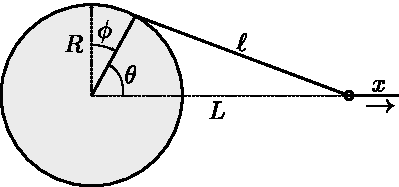
\includegraphics{geometry}
	\end{center}
	\caption{Geometric layout, and variables, for both the circular driver and this servo-controlled driver}
	\label{fig:circular}
\end{figure}

We decided to use geometry identical to that of the circular driver in figure \ref{fig:circular} but with a servomotor from a radio-control car steering system providing the motion, instead of driving the motion in a full circle at a constant angular velocity. 
Controlling a servo is very easy with a microcontroller: we chose a Teensy 4.0 for its combination of low price, high speed, breadboard-friendly form factor, and floating-point math capability.
By varying the maximum value of $\phi$, we can adjust the amplitude of $x$ on the fly. 

The only disadvantage remaining in this approach is the existence of harmonics arising from the cosine error in this geometry. 
Normally if one is driving a sinusoidal output with a microcontroller, the way to do it is to generate a look-up table (LUT) of values in the microcontroller memory.
The microcontroller looks up a value in the array, sets the output to that value, waits some time interval $\Delta t$, then looks up the next value and repeats the process. 
The frequency of the output waveform depends on $\Delta t$.
For a sinusoidal output, the look-up table would consist of values of sine (or cosine) evenly distributed over a complete period $T$.
But we didn't want the servo motion $\phi$ to be sinusoidal, we wanted $x$ to be sinusoidal!

\[ x = A \sin(\omega t) \]
This is equivalent to saying that (with a phase factor of $\pi$ depending on the sign of $x$)
\[ \ell(t) = \ell_o + A \sin(\omega t) \]
where 
\[ \ell_o \equiv \sqrt{R^2+L^2} \]
The servo is centered at $\phi=0$, so we want to find $\phi(t)$ such that $\ell(t)$ has the desired solution.
Start with the law of cosines:
\begin{eqnarray*} 
	\ell^2 &=& R^2 + L^2 - 2 R L \cos\theta\\
		&=& R^2 + L^2 - 2 R L \sin\phi\\
	\ell &=& \left[ R^2+L^2 - r R L \sin\phi \right]^{\frac{1}{2}} = \sqrt{R^2+L^2} + A \sin(\omega t)
\end{eqnarray*}

A few more careful steps of algebra give us an equation for the desired motion of the servo:
\begin{equation} \label{eq:phi}
	\phi(t) = \sin^{-1} \left[\frac{1}{2RL}\left(2\ell_o A\sin(\omega t) + A^2 \sin^2(\omega t)\right)\right]
\end{equation}

Equation \ref{eq:phi}\ is not particularly user-friendly, but one can check it for special cases. 
By geometric necessity $A<R$, so if $R\ll L$ then $\ell_o \approx L$, $\phi$ is small, and 
\[ \phi(t) \approx \frac{A}{R}\sin(\omega t) \]
as one would expect for this limiting-case geometry.
When $R$ is not small compared to $L$, one can consider the limiting case of $A \ll R$. 
In this case, the first term dominates and $\phi(t) \propto \sin(\omega t)$ as one would intuitively expect. 

For the general case, though, the microcontroller can move the servo through the curve described by equation \ref{eq:phi}\ just as easily as through a sine curve. 
Instead of building a LUT containing for $A\sin(\omega t)$ for each $t$ point, the microcontroller needs to build the LUT with values for $\phi(t)$.
The array will depend on $A$, so the LUT must be recalculated each time the amplitude is adjusted; but the Teensy microcontroller can recalculate the LUT values in a few microseconds.

\begin{figure}[ht]
	\begin{center}
		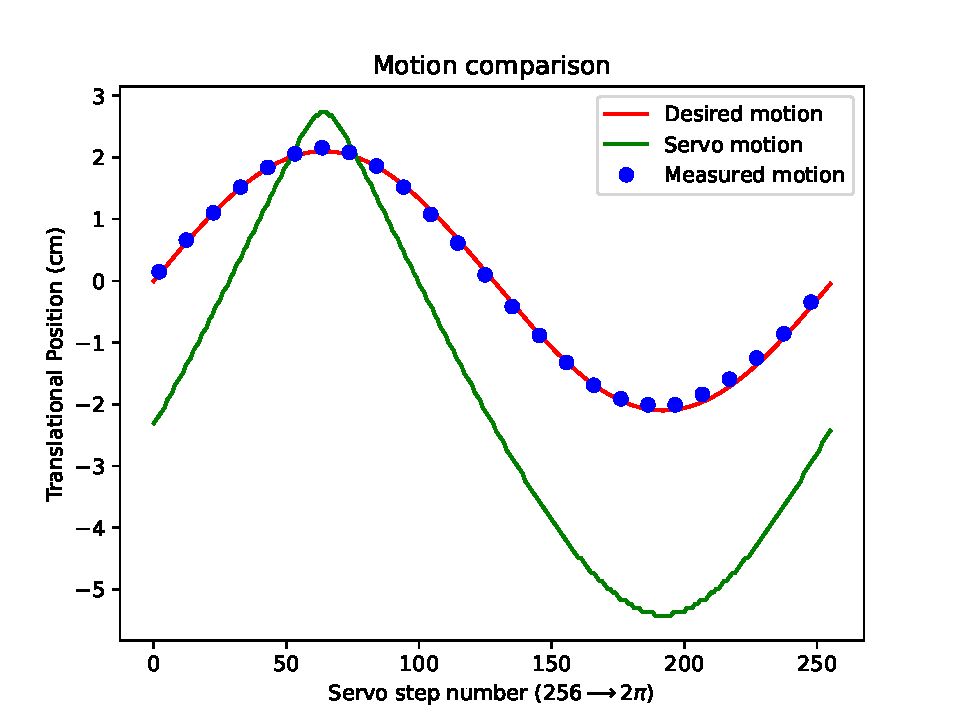
\includegraphics{comparison}
	\end{center}
	\caption{A plot of the servo motion $\phi$, as well as the resulting sinusoidal motion in $x$.}
	\label{fig:motion}
\end{figure}

\begin{figure}[ht]
	\begin{center}
		\includegraphics[width=6in]{device}
	\end{center}
	\caption{A photo of the completed device, showing the circuitboard, servo, and routing of the drive string.}
	\label{fig:device}
\end{figure}

Figure \ref{fig:motion} shows the non-sinusoidal motion of the servo end ($R\phi$) and the resulting sinusoidal motion of the output $x$, as measured by a Vernier GoDirect Sensor Cart\footnote{https://www.vernier.com/product/go-direct-sensor-cart/}.

The final construction step was to design a simple 3D-printed mount to hold the servo and the microcontroller board in place at one end of the dynamics track. 
See figure \ref{fig:device}.
For the fairly compact driver head we made, the improvement in the motion at maximum amplitude was an approximately 20dB decrease in the first harmonic compared to sinusoidal $\phi$.

There are several advantages to having a microcontroller-based mechanical driver such as this. 
A microcontroller can do much more than merely drive some constant frequency and amplitude. 
The program we wrote includes SCPI communications capability, so the device can be easily interfaced to LabVIEW, Python, or any other serial-capable programming language through the USB port on the Teensy 4.0 board.
For the purpose of the mechanics course demonstration that sparked this project, a simple python program to control frequency and amplitude sufficed to do what was needed. Other programs can be easily created to sweep through a range of frequencies for resonance curve analysis, or a range of amplitudes for investigations of chaotic oscillators.

\subsection*{Conclusions}
By calculating a non-sinusoidal arm motion for a servo in a situation in which cosine errors exist, we can use the cosine error to make the motion sinusoidal.
The microcontroller also provides computer control of frequency, amplitude, and (if desired) static position of the driver and allows easy control of the device via Python, LabVIEW, and other programming languages.

\subsection*{Want to build one?}
Microcontroller firmware, example Python control code, and 3D print files for this device are available on GitHub at https://github.com/EricAyars/Cart-driver

\end{document}

